\chapter{Allgemeine Begriffe}

\section{Konventionen}
Bereits Rechnungen in der "`gewöhnlichen"' Relativitätstheorie haben die Tendenz
unübersichtlich zu werden, das Einführen zusätzlicher Dimensionen hilft dabei
natürlich kaum.
Es ist deshalb an dieser Stelle nützlich einige Konventionen festzulegen. Im
Folgenden bezeichnet $n$ die Anzahl der Zusatzdimensionen.\footnote{Im Weiteren
meist $n=1$}

Die Metrik soll stets die Signatur $(1,3)$, bzw. $(1,3+n)$, insbesondere sind
die Zusatzdimensionen. Die meisten Rechnungen werden in lokalen Koordinaten
durchgeführt.
Wir beginnen die Indizierung bei 0, wobei die 0. Komponente mit der Zeit identifiziert wird.
Griechische Indices laufen über ersten vier Raum-Zeit Koordinaten
$\mu=0,\ldots,3\,$, lateinische über alle inklusive der
Zusatzkomponenten \footnote{Verwirrung bezüglich der gängigen Konvention
mit lateinischen Indices die Raumkomponenten zu benennen sollte dabei nicht
aufkommen.}, $i=0,\ldots,3+n\,$. Weiter verwenden wir die Einsteinsche
Summenkonvention, d.h. über paare von Indizes wird implizit summiert.

Im Zusammenhang mit Zusatzdimensionen tauchen Größen auf, die sowohl ein 4, als
auch ein $4+n$ dimensionales Pendant besitzen. Um diese von einander zu
unterscheiden, kennzeichnen wir die $4+n$ dimensionale Version mit einem
Zirkumflex.
Beispielsweise bezeichnen wir den $4+n$ dimensionalen Ricci-Tensor mit
$\tensor{\hat{R}}{_i_j}$. Mit $g$ bezeichnen wir die Determinante der Metrik.
\subsection*{Geometrisierte Einheiten}
Wir verwenden geometrisierte Einheiten, d.h. Einheiten in denen
$8\pi G=c=1$. Es verbleibt nur noch eine Längendimension.
\section{Modell einer höherdimensionalen Raumzeit}
In diesem Kapitel wollen wir ein möglichst allgemeines Modell einer
$d+4$-dimensionalen Raumzeit entwerfen. Häufig weisen Probleme in der Physik
Symmetrien auf, d.h. \ldots
Kontinuierliche Symmetrien lassen sich beispielsweise mithilfe besonderer
Gruppen, den so genannten \emph{Lie-Gruppen} beschreiben.
Bevor wir uns allerdings in die Konstruktion vertiefen ,geben wir ein einfaches
Beispiel für eine Symmetrie, dass uns auch im folgenden als Anschauungsobjekt
dienen wird.
\begin{beispiel}[Symmetrien eines Zylinders]
Wir betrachten einen Zylinder 
\begin{equation}
Z=\Reals\times\Sphere^1=\left\{(x,y,z)\in\Reals^3\,\Big|\,x^2+y^2=1\right\}\,,
\end{equation}
als Teilmenge des $\Reals^3$. 
Offensichtlich besitzt dieser zwei Symmetrien. Zum Einen wird er durch
Drehung um die $z$-Achse in sich selbst überführt (Rotationsinvarianz), zum
Anderen können wir den Ursprung entlang der $z$-Achse beliebig wählen
(Translationsinvarianz).
\end{beispiel}
Eine formale Beschreibung solcher Symmetrien bieten wie bereits angedeutet die
sogenannten Lie-Gruppen, Gruppen die zusätzlich eine Differenzierbare Struktur
besitzten.
\begin{definition}[Lie-Gruppe]

\end{definition}
\begin{bemerkung}
Der Zylinder $Z$ besitzt offensichtlich auch eine Spiegelsymmetrie bezüglich der
Koordinatenachsen. Dabei handelt es sich aber um eine diskrete Symmetrien,
welche sich nicht durch Lie-Gruppen beschreiben lassen.
\end{bemerkung}
% 
% \subsection{Vektoren und Tensoren}
% Riemann-Tensor, Ricci-Tensor, Geodätische.

%\subsection{Lie-Gruppen}
\begin{beispiel}[$SO(n)$]

\end{beispiel}
\section{Gruppenwirkungen}
In unserem Fall ist die Lie-Gruppe die die Operationen beschreibt die Gruppe der
Drehungen um die $z$-Achse. Diese wird mit $SO(2)$ bezeichnet, eine Darstellung
ergit sich beispielsweise durch Matrizen der Form
\begin{equation}
R(\alpha)=
\begin{pmatrix}
\cos\alpha&\sin\alpha&0\\
-\sin\alpha&\cos\alpha&0\\
0&0&1
\end{pmatrix}
\end{equation}
%TODO zusammenhang SO(2) und R/Z
Das diese Gruppe eine differenzierbare Struktur besitzt ist klar da die
Komponenten der Matrizen differenzierbar sind.
\begin{definition}[Lie-Gruppe]

\end{definition}

Gruppen können auf Mengen operieren.  Um die Diskussion allgemeiner zu gestalten definieren wir
Operationen allgemeiner Gruppen. 
Eine sinnvolle Operation einer Gruppe sollte mit den Gruppenoperationen
kompatibel sein. 
%TODO wedge product äußere Ableitung 
\begin{definition}[Gruppenwirkung]
Sei $G$ eine Gruppe, $X$ eine Menge. Eine Abbildung
\begin{equation}
\Phi:G\times X\to X\,,\quad (g,x)\mapsto\Phi_g(x)
\end{equation}
heißt \emph{Gruppenwirkung} von $G$ auf $X$, falls die folgende Eigenschaften
erfüllt sind
\begin{enumerate}
  \item \emph{Identität}: für das neutrale Element $e\in G$ gilt
  $\displaystyle\Phi_e=\id_X$
  \item \emph{Verträglichkeit}: $\displaystyle\Phi_{gh}=\Phi_g\circ\Phi_h$
\end{enumerate}
$X$ heißt dann auch $G$-Menge.
\end{definition}
Statt $\Phi_g(x)$ schreiben wir im folgenden kurz $g\gmal x$.
Ist die Gruppe $G$ eine Lie-Gruppe, $X=M$ eine Mannigfaltigkeit und $\Phi_g$
glatt, so spricht man von einer \emph{Lie-Gruppenwirkung}. $M$ heißt dann
auch $G$-Mannigfaltigkeit.
\begin{definition}
Sei $X$ eine $G$-Menge. Die Wirkung von $G$ heißt:
\begin{enumerate}
  \item \emph{eigentlich}, falls unter der Abbildung $\Gamma:
  G\times X\to X\times X\,,(g,x)\mapsto (g \gmal x,x)$, Urbilder kompakter
  Mengen kompakt sind
  \item \emph{(Fixpunkt-)frei}, falls nur die Identität Fixpunkte besitzt, d.h.
  aus $g\gmal x=x$, folgt $g=e$.
\end{enumerate}
\end{definition}
\begin{beispiel}[Wirkung von $\Reals/\Integers$ auf einem Zylinder]
Sei $G=(\Reals/\Integers,+)$, $Z$ wie oben. Eine Wirkung von $G$ auf $Z$ ist
erklärt durch
\begin{equation}
t.p= \begin{pmatrix}
\cos\left( 2\pi t\right)&\sin\left( 2\pi t\right)&0\\
-\sin\left( 2\pi t\right)&\cos\left( 2\pi t\right)&0\\
0&0&1
\end{pmatrix}p\,,\quad p\in Z\subset \Reals^3
\end{equation}
Wie man sich leicht klar macht ist die Wirkung glatt, frei und eigentlich.
%TODO eigentlich?
\end{beispiel}
\begin{figure}[!htbp]
\centering
\begin{tikzpicture}
\draw[-latex] (2,1)-- (-2,-1)  ;
\draw[-latex]  (-2,1)--(2,-1)  ;

\draw[fill=white,draw=none] (-1,4) -- (-1,0) arc (180:360:1cm and 0.5cm) -- (1,4) arc (-180:0:-1cm and 0.5cm) ;
\draw[fill=white,draw=none] (0,4) ellipse (1cm and 0.5cm);
\draw[-,thick, dashed] (0,-0.5) -- (0,4) ;
\draw[dashed] (2,1)-- (-2,-1)  ;
\draw[dashed]  (-2,1)--(2,-1)  ;
\draw[-,thick] (0,-1) -- (0,-0.5) ;
\node at (0,0) {\tiny\textbullet};
\node at (0,4) {\tiny\textbullet};
\draw[densely dashed] (-1,2) arc (180:0:1cm and 0.5cm);

\draw[fill=gray,fill opacity = 0.1,draw=none] (0,4) ellipse (1cm and 0.5cm);

\draw[fill=gray,fill opacity = 0.2] (-1,4) -- (-1,0) arc (180:360:1cm and 0.5cm) -- (1,4) arc (-180:0:-1cm and 0.5cm) ;
\draw[densely dashed] (-1,0) arc (180:0:1cm and 0.5cm);
\draw(-1,4) arc (180:0:1cm and 0.5cm);

\draw[densely dashed]  (-1,2) arc (-180:0:1cm and 0.5cm);
\draw[thick, red, -latex] (0,2) [partial ellipse=-60:-140:1cm and 0.5cm];
%\draw[thick, blue!80!black,-latex] (0.51,1.57)-- (0.51,3);
\node at (2.2,4) {$Z=\mathbb{R}\times\mathbb{S}^1$};
\node at (2+0.3,-1-0.2) {$y$};
\node at (-2+0.3,-1-0.2) {$x$};
\node at (0.3,5) {$z$};
\node at (0.5,1.25) {$p$};
\draw[-latex,thick] (0,4) -- (0,5) ;
\node at (0.51,1.57){\textbullet};
\end{tikzpicture}
\caption{Wirkung von $\Reals/\Integers$ auf dem Zylinder $Z$.}
\end{figure}
\section{Orbiträume}
Die Wirkung einer Gruppe definiert in natürlicher
Weise Äquivalenzklassen auf einer Mannigfaltigkeit, welche gerade diejenigen
Elemente enthalten, die sich durch $G$-Wirkung ineinander überführt werden.
Eine solche Äquivalenzklasse nennen wir Bahn oder Orbit. 
\begin{definition}[Orbit]
Sei $X$ eine $G$-Menge, $x\in X$, dann heißt die Menge
\begin{equation}
G \gmal x=\{g \gmal x\,|\,g\in G\}
\end{equation}
\emph{Orbit} von $x$. Als \emph{Orbitraum} bezeichnen wir die Menge aller Orbits
\begin{equation}
M/G=\{[x]=G.x\,|\,x\in M\}\,,
\end{equation}
versehen mit der Quotiententopologie, der gröbsten Topologie für die die
kanonische Projektion $x\mapsto [x]$ stetig ist.
\end{definition}
\begin{beispiel}[Orbits von $\Reals/\Integers$ auf $Z$]
Wenn wir wieder das Beispiel $G=\Reals/\Integers$, $M=Z$ heranziehen, so sind die Orbits gegeben durch
\begin{equation}
G.(0,0,z)=\left\{(\sin (2\pi t),\sin (2\pi t),z)\,,t \in
[0,1)\right\}\cong\Sphere^1\,.
\end{equation}
Der Orbitraum $M/G$ selbst ist offensichtlich diffeomorph zu $\Reals$. Der
Zylinder lässt sich also lokal als Produkt von Orbitraum und Orbit darstellen.
\end{beispiel}
\begin{figure}[!htbp]
\centering
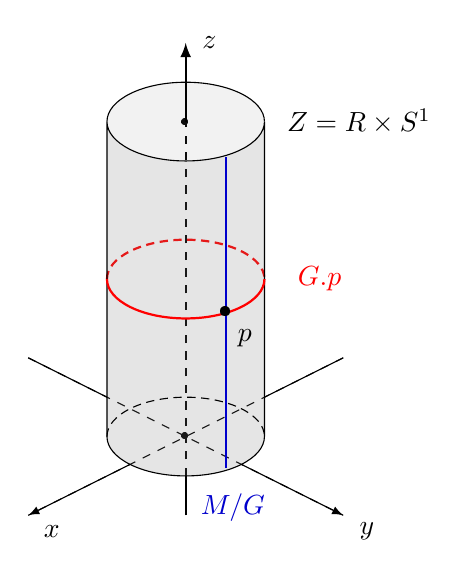
\begin{tikzpicture}
\draw[-latex] (2,1)-- (-2,-1)  ;
\draw[-latex]  (-2,1)--(2,-1)  ;

\draw[fill=white,draw=none] (-1,4) -- (-1,0) arc (180:360:1cm and 0.5cm) -- (1,4) arc (-180:0:-1cm and 0.5cm) ;
\draw[fill=white,draw=none] (0,4) ellipse (1cm and 0.5cm);
\draw[-,thick, dashed] (0,-0.5) -- (0,4) ;
\draw[dashed] (2,1)-- (-2,-1)  ;
\draw[dashed]  (-2,1)--(2,-1)  ;
\draw[-,thick] (0,-1) -- (0,-0.5) ;
\node at (0,0) {\tiny\textbullet};
\node at (0,4) {\tiny\textbullet};
\draw[densely dashed,red,thick] (-1,2) arc (180:0:1cm and 0.5cm);

\draw[fill=gray,fill opacity = 0.1,draw=none] (0,4) ellipse (1cm and 0.5cm);

\draw[fill=gray,fill opacity = 0.2] (-1,4) -- (-1,0) arc (180:360:1cm and 0.5cm) -- (1,4) arc (-180:0:-1cm and 0.5cm) ;
\draw[densely dashed] (-1,0) arc (180:0:1cm and 0.5cm);
\draw(-1,4) arc (180:0:1cm and 0.5cm);

\draw[red,thick]  (-1,2) arc (-180:0:1cm and 0.5cm);
% \draw[thick, red, -latex] (0,2) [partial ellipse=-60:-140:1cm and 0.5cm];
\draw[thick, blue!80!black] (0.51,-0.4)-- (0.51,3.55);
\node at (2.2,4) {$Z=\mathbb{R}\times\mathbb{S}^1$};
\node[red] at (1.7,2) {$G.p$};
\node[ blue!80!black] at (0.6,-0.9) {$M/G$};
\node at (2+0.3,-1-0.2) {$y$};
\node at (-2+0.3,-1-0.2) {$x$};
\node at (0.3,5) {$z$};
\node at (0.75,1.25) {$p$};
\draw[-latex,thick] (0,4) -- (0,5) ;
\node at (0.51,1.57){\textbullet};
;\end{tikzpicture}
\caption{Orbits der Wirkung der Gruppe $\Reals/\Integers$ auf $Z$.}
\end{figure}
% \begin{figure}
% \centering
% \begin{tikzpicture}
%
%    \draw[dashed] (1.3,-1.33) [partial ellipse= 90:270:0.5cm and 1cm];
%    \draw[dashed] (-1.3,-1.33) [partial ellipse=90:-90:0.5cm and 1cm];
%    \draw[thick, red,dashed] (-0,-1.5) [partial ellipse=270:90:0.4cm and 1cm];
%    \node[fill=white] at (0.7,-1.2) {$p$};
%   \node at (0.4,-1.5){\textbullet};
%    \node at (1.8,-1.3){\textbullet};
%    \node at (-1.8,-1.3){\textbullet};
% \fill[fill=gray,fill opacity = 0.2]  (-3.5,0) -- (0, 2.5)  -- (3.5,0);
% \fill[fill=gray,fill opacity = 0.2]  (-3.5,0) -- (0, -2.5)  -- (3.5,0);
% \draw[fill=gray,fill opacity = 0.2] (-3.5,0) .. controls (-3.5,2) and (-1.5,2.5) .. (0,2.5);
% \draw[xscale=-1,fill=gray,fill opacity = 0.2] (-3.5,0) .. controls (-3.5,2) and (-1.5,2.5) .. (0,2.5);
% \draw[rotate=180,fill=gray,fill opacity = 0.2] (-3.5,0) .. controls (-3.5,2) and (-1.5,2.5) .. (0,2.5);
% \draw[yscale=-1,fill=gray,fill opacity = 0.2] (-3.5,0) .. controls (-3.5,2) and (-1.5,2.5) .. (0,2.5);
%
% \draw (-2,.2) .. controls (-1.5,-0.3) and (-1,-0.5) .. (0,-.5) .. controls (1,-0.5) and (1.5,-0.3) .. (2,0.2);
%
% \draw[fill=white] (-1.75,0) .. controls (-1.5,0.3) and (-1,0.5) .. (0,.5) .. controls (1,0.5) and (1.5,0.3) .. (1.75,0);
% \draw[fill=white] (-1.75,0) .. controls (-1.5,-0.3) and (-1,-0.5) .. (0,-.5) .. controls (1,-0.5) and (1.5,-0.3) .. (1.75,0);
%   \draw[thick, red] (-0,-1.5) [partial ellipse=90:-90:0.4cm and 1cm];
%    \draw (1.3,-1.33) [partial ellipse=90:-90:0.5cm and 1.cm];
%
%     \draw (-1.3,-1.33)  [partial ellipse=270:90:0.5cm and 1cm];
%
%     \draw[dashed,  blue!80!black,thick] (-0,0) [partial ellipse=-180:0:3.5cm and 1.5cm];
%     \draw[thick,  blue!80!black] (-0,0) [partial ellipse=-110:-70:3.5cm and 1.5cm];
%   \node at (1,3) {$\mathbb{S}^1\times\mathbb{S}^1$};
% \end{tikzpicture}
% \end{figure}
Interessant sind insbesondere Fälle, in denen der Orbitraum selbst wieder eine
Mannigfaltigkeit darstellt. Dass dabei auch Probleme auftreten können, zeigt
folgendes 
\begin{beispiel}[Ein nicht Hausdorffscher Quotient
\cite{abraham1978foundations}] Sei $G=(\Reals,+)$, $M=\Reals$ und $G$ wirke auf
$M$ durch $t \gmal x=e^tx$.
Der Quotient $M/G$ enthält die drei Äquivalenzklassen $[-1],[0],[1]$, da die
Abbildung das Vorzeichen nicht ändert.
Die Quotiententopologie $\tau$ lässt sich explizit angeben:
\begin{equation}
\tau =\big\{\emptyset,\{[-1]\},\{[1]\},\{[-1],[1]\},M/G\big\}\,.
\end{equation}
Offensichtlich ist die einzige Menge, die $[0]$ enthält $M/G$. Die Elemente
$[0],[1]$ lassen sich damit nicht durch offene Mengen trennen, d.h. $(M/G,\tau)$
ist nicht Hausdorff.
\begin{figure}[!htbp]
\centering
\begin{tikzpicture}
\draw [dashed](-3,0)--(-2,0);
\draw [dashed](3,0)--(2,0);
\draw (-2,0)--(-0.3,0);
\draw (2,0)--(0.3,0);
\node at (-1,-2){\textbullet};
\node at (0,-2){\textbullet};
\node at (1,-2){\textbullet};
\node at (4,0){$M=\mathbb{R}$};
\node at (4,-2){$M/G$};
%\draw[<-] (-1,-3)--(-0.8,0);
%\draw (-1,-3)--(-2.5,-2.5);
%\draw (1,-3)--(0,0) --(2,0) --cycle;
%\draw (0,-3)--(0,0)  --cycle;
\node at (0,0){\textbullet};
\node at (-1,-2.5){$[-1]$};
\node at (0,-2.5){$[0]$};
\node at (1,-2.5){$[1]$};
\node at (0,.5){$G.0$};
\node at (-1.3,.5){$G.(-1)$};
\node at (1.3,.5){$G.1$};
\node at (-0.3,0){$)$};
\node at (0.3,0){$($};
\end{tikzpicture}
\caption{Konstruktion eines nicht Hausdorffschen Quotienten.}
\end{figure}
\end{beispiel}
Tatsächlich scheitert die Konstruktion daran, dass die Wirkung nicht eigentlich
ist, beispielsweise ist das Urbild $\Gamma^{-1}\big([0,1]\times
\{1\}\big)=(-\infty,0]\times \{1\}$ nicht kompakt.
Vielmehr lässt sich zeigen dass der Quotient genau dann Hausdorff ist, wenn die
Gruppe frei wirkt.
%TODO REF

Wir geben nun eine Charakterisierung, die solche pathologische
Fälle ausschließt.
% \begin{proposition}
% Sei $M$ eine $G$-Manigfaltigkeit, $R:=\big\{(g,g.x)|g\in G x\in M\big\}$ dann
% ist $R$ genau dann eine abgeschlossene Untermanigfaltigkeit von $M\times M$,
% wenn $M/G$ eine glatte Maigfaltigkeitsstruktur besitzt, sodass $\pi:M\to M/G$
% eine Submersion ist.
% \end{proposition}
% \begin{proof}
% Siehe R.Abraham "`Foundations of Mechanics"' \cite{abraham1978foundations}.
% \end{proof}
% \begin{theorem}[Slice Theorem]
% Ist $G$ eigentlich, so besitzt $M/G$ eine
% \end{theorem}
% Das Slice Theorem liefert, das falls $G$ kompakt und fixpunktfrei ist $M/G$ eine
% Manigfaltigkeitstruktur besitzt, bzw. sogar $M\to M/G$ ein $G$-Hauptfaserbündel
% ist.
% %http://math.stackexchange.com/questions/1315445/quotient-manifold-theorem-provides-a-fibrations
% Da die Gruppenwirkung differenzierbar ist lasst sich auch die Orbitkarte
% \begin{equation}
% \sigma_x:G\to M\,,\quad x\mapsto g \gmal x
% \end{equation}
% bei in der Identität differenzierbar. Man erhält so zu jedem $x\in M$ einen
% Vektor insgesammt erhält man ein Vektorfeld $V$ auf $M$.
%TODO Typen von Orbits. Maximale Orbits.
\begin{theorem}[Quotient Manifold Theorem \cite{lee2003smooth}]
Sei $G$ eine Lie-Gruppe, die glatt, frei und eigentlich auf einer glatten
Mannigfaltigkeit $M$ wirkt, dann ist der Orbitraum eine topologische
Mannigfaltigkeit der Dimension $\dim M/G=\dim M -\dim G$ und es existiert eine
eindeutige glatte Struktur sodass $\pi:M\to  M/G$ eine glatte Submersion ist.
\end{theorem}
\begin{korollar}
Sei $G$ eine Lie-Gruppe, die glatt, frei und eigentlich auf einer glatten
Mannigfaltigkeit $M$ wirkt. Dann ist $\pi:M\to M/G$ ein glattes Hauptfaserbündel,
mit Basis $M/G$ und typischer Faser $G$.
\end{korollar}
\section[Integration inv Fkt]{Integration auf Faserbündeln}
\begin{theorem}[Verallgemeinerter Fubini\label{th:fubini}]
Sei $M,N$, $m$ bzw. $n$-dimensionale, orientierbare Mannigfaltigkeiten, mit
$m\geq n$.
Sei $\varphi:M\to N$ glatt, $\omega$ eine $(m-n)$-Form auf $M$, sowie $\eta$
eine $n$-Form auf $N$. Sei $f:M\to \Reals$ Lebesgue integrabel, dann existiert
\begin{equation}
F(p)=\int_{\varphi^{-1}(p)}f\omega\,,
\end{equation}
das Integral entlang der Faser, für fast alle $p\in N$ und $F$ ist messbar. Es
gilt
\begin{equation}
\int_{M}f\omega\wedge\varphi^*\eta=\int_{N}F \eta\,.
\end{equation}
% Seien $M$, $N$ orientierbare Manigfaltigkeiten, $\pi$ die Projektion auf $M$
% bzw $N$, $\eta$, $\omega$ differentialformen auf $M$ bzw. $N$, $h:M\times N\to
% \Reals$ glatt, dann gilt
% \begin{equation}
% \int_{M\times N} h\pi_1^\star\eta\wedge\pi_2^\star\omega
% =\int_M g\eta\,,\quad g(p):=\int_N h(p,\cdot)\omega\,.
% \end{equation}
\end{theorem}
\begin{proof}
Sulantke und Wintgen
%Polynomial Convexity Edgar Lee Stout
\end{proof}
\begin{bemerkung}
Bei \autoref{th:fubini} handelt es sich um eine Verallgemeinerung des aus der
Analysis bekannten Satzes von Fubini. 
Sei $M=\Reals^m$, $N=\Reals^n$, und 
\begin{align*}
  \pi :M &\to N\\
  (x_1,\dots,x_n,y_1,\dots,y_k) &\mapsto (x_1,\dots,x_n)\,.
\end{align*}
Wir definieren Differentialformen auf $N$ bzw. $M$ durch 
$\omega=\dif{x}^1\wedge\cdots\wedge\dif{x}^n$ und
$\eta=\dif{x}^{n+1}\wedge\cdots\wedge\dif{x}^m$.
Nach\autoref{th:fubini}gilt
\begin{equation}
\begin{split}
\int_{\Reals^m} f\dif{}^m x &= \int_{\Reals^m}
f\dif{x}^1\wedge\cdots\wedge\dif{x}^n\wedge\dif{x}^{n+1}\wedge\cdots\wedge\dif{x}^m\\
&= \int_{\Reals^m}f\,\omega\wedge\pi^*\eta\\
&= \int_{\Reals^n}\left(\int_{\pi^{-1}(x)}f\,\omega\right)\eta\\
&= \int_{\Reals^n}\left(\int_{\{x\}\times\Reals^{(m-n)}}f\,\omega\right)\eta\,,
\end{split}
\end{equation}
was der bekannten Formel entspricht.
\end{bemerkung}
Ein interessantes Resultat ergibt sich wenn wir Funktionen betrachten, die
entlang der Fasern $\pi^{-1}(x)$ konstant sind.
\begin{definition}
Sei $X$ eine $G$-Menge, $Y$ eine Menge, $f:X\to Y$ mit
\begin{equation}
f(g\gmal p)=f(p)\,,\quad \forall g\in G\,,p\in E\,,
\end{equation}
dann heißt $f$ $G$-invariant.
\end{definition}
Sei $G$ eine Liegruppe mit endlichem Volumen $\vol(G):=\int_G\dif h<\infty$. 
Wir betrachten ein $G$-Hauptfaserbündel $\pi: E\to M$,
ausgestattet mit einer $G$-invarianten (pseudo-)riemannschen Metrik $g$. 
Die Abbildung $f:E\to \Reals$ sei $G$-invariant und integrierbar. Dann gilt nach
\autoref{th:fubini}
\begin{equation}
\begin{split}
\int_E f\sqrt{g}\dif{}\hat{x}&=\int_{M}\int_{G}f\sqrt{g}\dif^{}h \dif x\\
&=\int_{M}f\sqrt{g}\int_{G}\dif^{}h \dif x\\
&=\vol(G)\int_{M}f\sqrt{g} \dif x\\
\end{split}
\end{equation}
Die Integration über den Totalraum $E$ kann also mit einer Integration über die
Basis $M$ identifiziert werden.
% Eine
% Tivialisierung einer offenen Menge $U\subset M=E/G$, ist ein Homoemorphismus
% \begin{equation}
% \Psi:\pi^{-1}(U)\to U\times G\,.
% \end{equation}
% Wir definieren eine Abbildung $\tilde{f}: M\to\mathrm{R}$
% \begin{equation}
% \tilde{f}\left(x\right):=\left(f\circ \Psi^{-1}\right)(x,e)\,.
% \end{equation}
% % Diese ist wohldefiniert, denn
% % \begin{equation}
% % \begin{split}
% % f\left(\Psi^{-1}(x,h)\right)&=f\left(\Psi^{-1}(x,h.e)\right)\\
% % &=f\left(h.\Psi^{-1}(x,e)\right)\\
% % &=f\left(\Psi^{-1}(x,e)\right)\,.
% % \end{split}
% % \end{equation}
% Damit gilt
% \begin{equation}
% \begin{split}
% \int_{\pi^{-1}(U)}f(x)\dif x&=
% \int_{\Psi\left(\pi^{-1}(U)\right)}\left[f\circ\Psi^{-1}\right](y,h)\dif y
% \dif h\\
% &=
% \int_{U\times G}\left[f\circ\Psi^{-1}\right](y,h)\dif y
% \dif h\\
% &=\int_G\int_{U}\tilde{f}\left(y\right)\dif y
% \dif h\\
% &=\vol (G)\int_{U}\tilde{f}\left(y\right)\dif y\,,\label{eq:Intprod}
% \end{split}
% \end{equation}
% Eine anschauliche Betrachtung $\tilde{f}$ als Mittelung der makroskopischen Funktion $f$ über die Zusatzdimension auffassen.
% Phsikalisch liegt ein solcher Fall vor, falls die Auflösung einer Messung zu
% gering ist um die kompakte Dimension zu beobachten. Bisher konnten kompakte
% Zusatzdimensionen nicht beobachtet werden, neue Erkentnisse bringt
% möglicherweise der 2015 gestarteten Lauf des Large Hadron Coliders am CERN. Die
% lokalen Trivialisierungen überdecken $M$, damit lassen sich auch Integrale auf dem gesammten Raum auf
% Integrale von der Form \eqref{eq:Intprod} zurückführen insbesondere gilt für die
% $G$-invariante Funktion $f\sqrt{g}$
% \begin{equation}
% \int_{E}f(x)\sqrt{g(x)}\dif x=\vol
% (G)\int_{M}\tilde{f}\left(y\right)\sqrt{\tilde{g}(y)}\dif y
% \end{equation}
% wobei $\tilde{g}(y)=\left[g\circ\Psi^{-1}\right](y,h)$. Im folgenden lassen wir
% die Tilden weg und identifizieren die Ausdrücke stillschweigend miteinander.
% Wir beenden dieses Kapitel mit einem Beispiel, der sogenannten
%\emph{ADM-decomposition}.
\begin{beispiel}[ADM-decomposition]
 
 \end{beispiel}
\section{Ein Variationsprinzip}
Variationsprinzipien stellen eine elegante Möglichkeit dar, physikalische
Theorien zu formulieren. Die Physik wird dabei durch einen Satz
von Parametern bzw. Funktionen beschrieben die in gewisser Weise "`optimal"' sind. 
Wir orientieren uns in diesem Kapitel an den Ausführungen von \name{R.Wald}
\cite[s.454 ff]{wald2010general}.
Im folgenden bezeichnet \emph{Feld} allgemein ein Tensorfeld, wobei wir den
Grad nicht angeben, sowie \emph{Feldkonfiguration} ein Tupel solcher
Feldern. 
Wir wollen nun einen Formalismus entwickeln, der es erlaubt ein Funktional, nach
einer Funktion abzuleiten, was es ermöglicht Extremalbedingunen in Analogie zur
klassischen Analysis zu formulieren.
\begin{definition}[Funktionalableitung] 
\label{def:Funktionalableitung}
Sei $M$ eine Mannigfaltigkeit,
$X\subseteq C^\infty(M)$ ein Funktionenraum. Sei $I:X\to \Reals$ ein Funktional,
$\left(f_\lambda\right)_{\lambda\in \Reals}\subseteq X$, eine einparametrige
Familie von Funktionen, die differenzierbar von $\lambda$ abhängt.
Angenommen $\lambda\mapsto I\left[f_\lambda\right]$ ist für alle solche Familien
in $\lambda=0$ differenzierbar und es existiert eine Distribution $g$, sodass
 \begin{equation}
 \dod{}{\lambda}\Big|_{\lambda=0}I[f_\lambda]
 =\int_M g\dod{}{\lambda}\Big|_{\lambda=0}f_\lambda\dif x\,
 \label{eq:Vardiff1}
 \end{equation}
 für alle Familien $f_\lambda$, dann heißt
 \begin{equation}
\frac{\delta{I}}{\delta{f}}\bigg|_{f_0}:=g
 \end{equation}
 \emph{Variationsableitung} von $I$ in $f_0$.
\end{definition}
\begin{bemerkung}
Der Begriff der Variationsableitung lässt sich auf natürliche Weise auf 
Funktionale von Feldern oder allgemeiner Feldkonfigurationen erweitern wenn wir
in \autoref{def:Funktionalableitung} Funktion durch Feld bzw. Feldkonfiguration
ersetzen, sowie  in \eqref{eq:Vardiff1} die Tensorindizes der
Felder $g$ und $f_\lambda$ kontrahieren.
\end{bemerkung}
\subsection{Der Lagrangeformalismus}
Einen wichtigen Spezialfall stellen Funktionale dar, die durch eine
lokale\footnote{"`Lokal"' bezieht sich anschaulich darauf, dass der Wert des
Integranden in $x\in M$ lediglich von diesem Punkt abhängt.} Funktion
${L:\Reals^3\to \Reals}$ charakterisiert werden, d.h. \footnote{Hier
und im folgenden bezeichnet $\partial_i$ eine Differentiation nach der $i$-ten
Koordinate.}
\begin{equation}
I[f]=\int_M L\left(f(x),\partial_i f(x),x\right)\dif x\,.
\end{equation}
Die Funktion $L$ heißt dabei auch \emph{Lagrange-Funktion} oder auch
\emph{Lagrangian}.
Die Variation des Funktionals $I$ führt in diesem Fall auf
\begin{equation}
\begin{split}
\dod{I}{\lambda}
&=\int_M\dod{}{\lambda}L(f_\lambda,\partial_i
f_\lambda,x)\dif x\\
&=\int_M\dpd{L}{ f}\dpd{ f_\lambda}{\lambda}
+\dpd{L}{(\partial_i f)}\dpd{(\partial_i f_\lambda)}{\lambda}\dif x\\
&=\int_M\dpd{L}{ f}\dpd{ f_\lambda}{\lambda}
+\dpd{L}{(\partial_i f)}\partial_i\left(\dpd{
f_\lambda}{\lambda}\right)\dif x\\
&=\int_M\left\{\dpd{L}{ f}
-\partial_i\left[\dpd{L}{(\partial_i f)}\right]\right\}\dpd{
f_\lambda}{\lambda}\dif x +\int_{\partial
M}\dpd{L}{(\partial_i f)}\dpd{
f_\lambda}{\lambda}n_i\dif\sigma\,,
\end{split}
\end{equation}
dabei haben wir im dritten Schritt die Vertauschbarkeit
der partiellen Ableitungen nach dem Satz von Schwarz, sowie im letzten
partielle Integration verwendet, wobei $n_i$ ein Vektorfeld normal zu $\partial M$
bezeichnet, wir nehmen dabei an, dass die Mannigfaltigkeit orientierbar ist,
d.h.\ ein solches Normalenfeld existiert.
%TODO partielle Integration auf MF
Häufig beschränkt man sich auf kompakte Variationen, d.h. für alle $\lambda$ ist
$f_\lambda(x)=f_0(x)$, bzw. $\pd{ f_\lambda}{\lambda}=0$ auf $\partial M$. Die
Integration über den Rand verschwindet damit und es ergibt sich
\begin{equation}
\begin{split}
\dod{I}{\lambda}
&=\int_M\left\{\dpd{L}{ f}
-\partial_i\left[\dpd{L}{(\partial_i f)}\right]\right\}\dpd{
f_\lambda}{\lambda}\dif x\,.
\end{split}
\end{equation}
Geht man nun davon aus, dass eine bestimmte Funktion $f$ das Funktional
$I$ minimiert, d.h. $\od{I}{\lambda}=0$ für eine beliebige Variation, 
so muss nach dem Lemma der Variationsrechnung
\begin{equation}
\dpd{L}{f}
-\partial_i\left[\dpd{L}{(\partial_i f)}\right]=0\,,
\end{equation}
die \emph{Euler-Lagrange-Gleichung}. Diese spielt eine bedeutende Rolle in der
theoretischen Mechanik. Der Formalismus eine Funktion als Extremum eines
Funktionals zu wählen ist unter dem Namen \emph{Lagrange-Formalismus} bekannt und lässt sich auf
natürliche Weise auf Feldkonfigurationen $\Psi$ verallgemeinern. Das
Funktional ist dann von der Form
\begin{equation}
I[\Psi]=\int_M L\left(\Psi,\partial_i \Psi,x\right)\dif x
\end{equation}
und die resultierenden Euler-Lagrange-Gleichungen lauten
\begin{equation}
\dpd{L}{\Psi}
-\partial_i\left[\dpd{L}{(\partial_i\Psi)}\right]=0\,,
\end{equation}
wobei dieser Ausdruck als eine Gleichung pro
unabhängige Feldkomponente zu interpretieren ist.
\begin{beispiel}[Spin-1 Felder]
Als Beispiel betrachten wir das elektromagnetische Feld, welches durch eine
1-Form $A$ beschrieben werden kann. In lokalen Koordinaten wird $A$
durch Funktionen $A_0,\dots,A_3$ beschreiben. Nehmen wir an der Lagrange
Funktion $L$ sei gegeben durch \footnote{Diese muss nicht "`geraten"'
werden, vielmehr handelt es sich um den allgemeinste solche Funktion die
gewissen Symmetrien genügt. }
\begin{equation}
L\left(A_\alpha(x),\nabla_\beta
A_\alpha(x),x\right)=-\frac{1}{4}\tensor{F}{_\mu_\nu}\tensor{F}{^\mu^\nu}\,.
\end{equation}
mit
$\tensor{F}{_\mu_\nu}=\tensor{\partial}{_\mu}\tensor{A}{_\nu}-\tensor{\partial}{_\nu}\tensor{A}{_\mu}$.
Unabhängigkeit der Felder bedeutet
\begin{equation}
\pd{\tensor{F}{_\mu_\nu}}{(\tensor{\partial}{_\alpha}\tensor{A}{_\beta})}
=\tensor*{\delta}{^\alpha_\mu}\tensor*{\delta}{^\beta_\nu}\,.
\end{equation}
Damit können wir $L$ nach $\tensor{A}{_\mu}$ differenzieren:
\begin{equation}
\begin{split}
\dpd{L}{(\tensor{\partial}{_\alpha}\tensor{A}{_\beta})}
&=\dpd{\tensor{F}{_\mu_\nu}}{(\tensor{\partial}{_\alpha}\tensor{A}{_\beta})}\tensor{F}{^\mu^\nu}
+\dpd{\tensor{F}{^\mu^\nu}}{(\tensor{\partial}{_\alpha}\tensor{A}{_\beta})}\tensor{F}{_\mu_\nu}
\\
&=\dpd{\tensor{F}{_\mu_\nu}}{(\tensor{\partial}{_\alpha}\tensor{A}{_\beta})}\tensor{F}{^\mu^\nu}
+\dpd{(\tensor{g}{^\mu^\delta}\tensor{g}{^\mu^\gamma}\tensor{F}{_\delta_\gamma})}{(\tensor{\partial}{_\alpha}\tensor{A}{_\beta})}\tensor{F}{_\mu_\nu}
\\
&=\dpd{\tensor{F}{_\mu_\nu}}{(\tensor{\partial}{_\alpha}\tensor{A}{_\beta})}\tensor{F}{^\mu^\nu}
+\dpd{\tensor{F}{_\delta_\gamma}}{(\tensor{\partial}{_\alpha}\tensor{A}{_\beta})}\tensor{g}{^\mu^\delta}\tensor{g}{^\mu^\gamma}\tensor{F}{_\mu_\nu}
\\
&=2\dpd{\tensor{F}{_\mu_\nu}}{(\tensor{\partial}{_\alpha}\tensor{A}{_\beta})}\tensor{F}{^\mu^\nu}\\
&=2\tensor*{\delta}{^\alpha_\mu}\tensor*{\delta}{^\beta_\nu}\tensor{F}{^\mu^\nu}\\
&=2\tensor{F}{^\alpha^\beta}\,.
\end{split}
\end{equation}
Mit $\pd{L}{\tensor{A}{_\alpha}}=0$ lauten die Euler-Lagrange-Gleichungen
\begin{equation}
\partial_\alpha\tensor{F}{^\alpha^\beta}=0\,,
\end{equation}
die Maxwell Gleichungen die in Kapitel ??? vorgestellt werden
%TODO 
\end{beispiel}
% \begin{equation}
% \begin{split}
% \dod{S}{\lambda}
% &=\int_M\left\{\dpd{L}{\Psi}
% -\partial_i\left[\dpd{L}{(\partial_i\Psi)}\right]\right\}\dpd{\Psi}{\lambda}\dif
% x\,.
% \end{split}
% \end{equation}
% Identifizieren wir die Felder mit ihren lokalen Darstellungen im $\Reals^m$ und
% bezeichnet $d=\dim M$ die Dimension der Mannigfaltigkeit, so können wir
% $L$ als Funktion
% \begin{equation}
% L:\Reals^m\times\Reals^{m\cdot d}\times \Reals^d\to\Reals 
% \end{equation}
% auffassen. Damit ist klar was unter den Ausdrücken 
% \begin{equation}
% \dpd{L}{\Psi},\dpd{L}{(\partial_i\Psi)},\dots
% \end{equation}
% zu verstehen ist. Die Variation des Funktionals $I$ führt auf 
% \begin{equation}
% \begin{split}
% \dod{I}{\lambda}
% &=\int_M\dod{L}{\lambda}\dif x\\
% &=\int_M\dpd{L}{\Psi}\dpd{\Psi}{\lambda}
% +\dpd{L}{(\partial_i\Psi)}\dpd{(\partial_i\Psi)}{\lambda}\dif x\\
% &=\int_M\dpd{L}{\Psi}\dpd{\Psi}{\lambda}
% +\dpd{L}{(\partial_i\Psi)}\partial_i\left[\dpd{\Psi}{\lambda}\right]\dif
% x\\
% &=\int_M\left\{\dpd{L}{\Psi}
% -\partial_i\left[\dpd{L}{(\partial_i\Psi)}\right]\right\}\dpd{\Psi}{\lambda}\dif x
% +\int_{\partial
% M}\dpd{L}{(\partial_i\Psi)}\dpd{\Psi}{\lambda}n_i\dif\sigma\,,
% \end{split}
% \end{equation}
% dabei wurde im zweiten Schritt die Kettenregel im dritten die Vertauschbarkeit
% der partiellen Ableitungen und im letzten partielle Integration verwendet. Die
% Integration über den Rand der Mannigfaltigkeit $\partial M$ wird typischerweise zu null angenommen, was sich beispielsweise dadurch begründen
% lässt, dass die Variation $\dpd{\Psi}{\lambda}$ auf dem Rand verschwindet. Dann
% ergibt sich
% \begin{equation}
% \begin{split}
% \dod{S}{\lambda}
% &=\int_M\left\{\dpd{L}{\Psi}
% -\partial_i\left[\dpd{L}{(\partial_i\Psi)}\right]\right\}\dpd{\Psi}{\lambda}\dif
% x\,.
% \end{split}
% \end{equation}
% Geht man nun davon aus, dass eine bestimmte Konfiguration $\Psi$ das Funktional
% $S$ minimiert, d.h. $\dod{S}{\lambda}=0$ für eine beliebige Variation.
% Dann muss nach dem Lemma der Variationsrechnung 
% \begin{equation}
% \dpd{L}{\Psi}
% -\partial_i\left[\dpd{L}{(\partial_i\Psi)}\right]=0
% \end{equation}

\begin{definition}[Tensordichte]
Eine Tensordichte $\mathcal{T}$ vom Gewicht $w$
\end{definition}
Wirkungsintegral, Lagrangedichte, Lokalität
\begin{beispiel}[Levi-Civita-Symbol]
\end{beispiel}
% \begin{definition}[Variationsableitung]
% Sei $\Omega$ ein normierter Vektorraum, $I:\Omega\to \Reals$ ein Funktional,
% das auf einer offenen Umgebung von $x\in \Omega$ definiert ist $h\in \Omega$,
% dann heißt der Ausdruck
% \begin{equation}
% \delta_h I=\lim_{\varepsilon\to 0} \frac{I(x+\varepsilon h)-I(x)}{\varepsilon}
% \end{equation}
% \emph{G\^ateaux Ableitung} von $I$, bzw. \emph{erste Variation} von $I$ nach
% $h$, sofern er existiert.
% % es wird nach einem Feld gesucht nicht nach einem "`optimalen"' Weg, quasi
% % unendlichdimensionale Form
% % https://en.wikipedia.org/wiki/Lagrangian_system
% \end{definition}
% \begin{beispiel}[Lokale Funktionale]
% Sei $I$ ein Lokales Funktional 
% \begin{equation}
% I(f)=\int_M \mathcal{I}[f(x),\partial_i f(x),x]\dif x
% \end{equation}
% \begin{equation}
% \begin{split}
% \mathcal{I}[f(x)+\varepsilon h(x),\partial_i
% f(x)+\varepsilon\partial_i h,x]
% &=\dpd{\mathcal{I}}{f}h+\dpd{\mathcal{I}}{(\partial_i
% f)}\partial_i h
% \end{split}
% \end{equation}
%\end{beispiel}
% \begin{lemma}[Variationsprinzip]
% Extremum $\implies\delta_h I = 0$
% \end{lemma}
% \subsubsection{Skalarfelder (Spin-0)}
% \begin{equation}
% \mathcal{L}\left[\phi(x),\nabla_\alpha\phi(x),x\right]=
% \end{equation}
% \subsubsection{Vektorfelder (Spin-1)}
% \begin{equation}
% \mathcal{L}\left[A_\alpha(x),\nabla_\beta
% A_\alpha(x),x\right]=-\frac{1}{4}\tensor{F}{_\mu_\nu}\tensor{F}{^\mu^\nu}\,.
% \end{equation}
%https://en.wikipedia.org/wiki/Euler%E2%80%93Lagrange_equation
%https://en.wikipedia.org/wiki/Functional_derivative#cite_note-2

% Fibred manifold vs principal bundle (spezialfall\ldots)
% In topology, the words fiber (Faser in German) and fiber space (gefaserter Raum)
% appeared for the first time in a paper by Seifert in 1932
% Seifert, H. (1932). "Topologie dreidimensionaler geschlossener Räume". Acta
% Math. (in French) 60: 147–238. doi:10.1007/bf02398271.
